%%% Hlavní soubor. Zde se definují základní parametry a odkazuje se na ostatní části. %%%

%% Verze pro jednostranný tisk:
% Okraje: levý 40mm, pravý 25mm, horní a dolní 25mm
% (ale pozor, LaTeX si sám přidává 1in)
\documentclass[12pt,a4paper]{report}
\setlength\textwidth{145mm}
\setlength\textheight{247mm}
\setlength\oddsidemargin{15mm}
\setlength\evensidemargin{15mm}
\setlength\topmargin{0mm}
\setlength\headsep{0mm}
\setlength\headheight{0mm}
% \openright zařídí, aby následující text začínal na pravé straně knihy
\let\openright=\clearpage

%% Pokud tiskneme oboustranně:
% \documentclass[12pt,a4paper,twoside,openright]{report}
% \setlength\textwidth{145mm}
% \setlength\textheight{247mm}
% \setlength\oddsidemargin{14.2mm}
% \setlength\evensidemargin{0mm}
% \setlength\topmargin{0mm}
% \setlength\headsep{0mm}
% \setlength\headheight{0mm}
% \let\openright=\cleardoublepage

%% Vytváříme PDF/A-2u
\usepackage[a-2u]{pdfx}

%% Přepneme na českou sazbu a fonty Latin Modern
\usepackage[czech]{babel}
\usepackage{lmodern}
\usepackage[T1]{fontenc}
\usepackage{textcomp}

%% Použité kódování znaků: obvykle latin2, cp1250 nebo utf8:
\usepackage[utf8]{inputenc}

%%% Další užitečné balíčky (jsou součástí běžných distribucí LaTeXu)
\usepackage{amsmath}        % rozšíření pro sazbu matematiky
\usepackage{amsfonts}       % matematické fonty
\usepackage{amsthm}         % sazba vět, definic apod.
\usepackage{bbding}         % balíček s nejrůznějšími symboly
			    % (čtverečky, hvězdičky, tužtičky, nůžtičky, ...)
\usepackage{bm}             % tučné symboly (příkaz \bm)
\usepackage{graphicx}       % vkládání obrázků
\usepackage{fancyvrb}       % vylepšené prostředí pro strojové písmo
\usepackage{indentfirst}    % zavede odsazení 1. odstavce kapitoly
\usepackage{natbib}         % zajištuje možnost odkazovat na literaturu
			    % stylem AUTOR (ROK), resp. AUTOR [ČÍSLO]
\usepackage[nottoc]{tocbibind} % zajistí přidání seznamu literatury,
                            % obrázků a tabulek do obsahu
\usepackage{icomma}         % inteligetní čárka v matematickém módu
\usepackage{dcolumn}        % lepší zarovnání sloupců v tabulkách
\usepackage{booktabs}       % lepší vodorovné linky v tabulkách
\usepackage{paralist}       % lepší enumerate a itemize
\usepackage{xcolor}         % barevná sazba

%%% Údaje o práci

% Název práce v jazyce práce (přesně podle zadání)
\def\NazevPrace{Závěrečná zpráva z ročníkového projektu}

% Název práce v angličtině
\def\NazevPraceEN{Name of thesis}

% Jméno autora
\def\AutorPrace{Jméno Příjmení}

% Rok odevzdání
\def\RokOdevzdani{2024}

% Název katedry nebo ústavu, kde byla práce oficiálně zadána
% (dle Organizační struktury MFF UK, případně plný název pracoviště mimo MFF)
\def\Katedra{Název katedry nebo ústavu}
\def\KatedraEN{Name of the department}

% Jedná se o katedru (department) nebo o ústav (institute)?
\def\TypPracoviste{Katedra}
\def\TypPracovisteEN{Department}

% Vedoucí práce: Jméno a příjmení s~tituly
\def\Vedouci{Vedoucí práce}

% Pracoviště vedoucího (opět dle Organizační struktury MFF)
\def\KatedraVedouciho{katedra}
\def\KatedraVedoucihoEN{department}

% Studijní program a obor
\def\StudijniProgram{studijní program}
\def\StudijniObor{studijní obor}

% Nepovinné poděkování (vedoucímu práce, konzultantovi, tomu, kdo
% zapůjčil software, literaturu apod.)
\def\Podekovani{%
Poděkování.
}

% Abstrakt (doporučený rozsah cca 80-200 slov; nejedná se o zadání práce)
\def\Abstrakt{%
Abstrakt.
}
\def\AbstraktEN{%
Abstract.
}

% 3 až 5 klíčových slov (doporučeno), každé uzavřeno ve složených závorkách
\def\KlicovaSlova{%
{klíčová} {slova}
}
\def\KlicovaSlovaEN{%
{key} {words}
}

%% Balíček hyperref, kterým jdou vyrábět klikací odkazy v PDF,
%% ale hlavně ho používáme k uložení metadat do PDF (včetně obsahu).
%% Většinu nastavítek přednastaví balíček pdfx.
\hypersetup{unicode}
\hypersetup{breaklinks=true}

%% Definice různých užitečných maker (viz popis uvnitř souboru)
%%% Tento soubor obsahuje definice různých užitečných maker a prostředí %%%
%%% Další makra připisujte sem, ať nepřekáží v ostatních souborech.     %%%

%%% Drobné úpravy stylu

% Tato makra přesvědčují mírně ošklivým trikem LaTeX, aby hlavičky kapitol
% sázel příčetněji a nevynechával nad nimi spoustu místa. Směle ignorujte.
\makeatletter
\def\@makechapterhead#1{
  {\parindent \z@ \raggedright \normalfont
   \Huge\bfseries \thechapter. #1
   \par\nobreak
   \vskip 20\p@
}}
\def\@makeschapterhead#1{
  {\parindent \z@ \raggedright \normalfont
   \Huge\bfseries #1
   \par\nobreak
   \vskip 20\p@
}}
\makeatother

% Toto makro definuje kapitolu, která není očíslovaná, ale je uvedena v obsahu.
\def\chapwithtoc#1{
\chapter*{#1}
\addcontentsline{toc}{chapter}{#1}
}

% Trochu volnější nastavení dělení slov, než je default.
\lefthyphenmin=2
\righthyphenmin=2

% Zapne černé "slimáky" na koncích řádků, které přetekly, abychom si
% jich lépe všimli.
\overfullrule=1mm

%%% Makra pro definice, věty, tvrzení, příklady, ... (vyžaduje baliček amsthm)

\theoremstyle{plain}
\newtheorem{veta}{Věta}
\newtheorem{lemma}[veta]{Lemma}
\newtheorem{tvrz}[veta]{Tvrzení}

\theoremstyle{plain}
\newtheorem{definice}{Definice}

\theoremstyle{remark}
\newtheorem*{dusl}{Důsledek}
\newtheorem*{pozn}{Poznámka}
\newtheorem*{prikl}{Příklad}

%%% Prostředí pro důkazy

\newenvironment{dukaz}{
  \par\medskip\noindent
  \textit{Důkaz}.
}{
\newline
\rightline{$\qedsymbol$}
}

%%% Prostředí pro sazbu kódu, případně vstupu/výstupu počítačových
%%% programů. (Vyžaduje balíček fancyvrb -- fancy verbatim.)

\DefineVerbatimEnvironment{code}{Verbatim}{fontsize=\small, frame=single}

%%% Prostor reálných, resp. přirozených čísel
\newcommand{\R}{\mathbb{R}}
\newcommand{\N}{\mathbb{N}}

%%% Užitečné operátory pro statistiku a pravděpodobnost
\DeclareMathOperator{\pr}{\textsf{P}}
\DeclareMathOperator{\E}{\textsf{E}\,}
\DeclareMathOperator{\var}{\textrm{var}}
\DeclareMathOperator{\sd}{\textrm{sd}}

%%% Příkaz pro transpozici vektoru/matice
\newcommand{\T}[1]{#1^\top}

%%% Vychytávky pro matematiku
\newcommand{\goto}{\rightarrow}
\newcommand{\gotop}{\stackrel{P}{\longrightarrow}}
\newcommand{\maon}[1]{o(n^{#1})}
\newcommand{\abs}[1]{\left|{#1}\right|}
\newcommand{\dint}{\int_0^\tau\!\!\int_0^\tau}
\newcommand{\isqr}[1]{\frac{1}{\sqrt{#1}}}

%%% Vychytávky pro tabulky
\newcommand{\pulrad}[1]{\raisebox{1.5ex}[0pt]{#1}}
\newcommand{\mc}[1]{\multicolumn{1}{c}{#1}}


%% Titulní strana a různé povinné informační strany
\begin{document}
%%% Titulní strana práce a další povinné informační strany

%%% Titulní strana práce

\pagestyle{empty}
\hypersetup{pageanchor=false}

\begin{center}

\centerline{\mbox{
\includegraphics[width=166mm]{../img/logo-cs.pdf}}}

\vspace{-8mm}
\vfill

{\bf\Large ROČNÍKOVÁ PRÁCE}

\vfill

{\LARGE\AutorPrace}

\vspace{15mm}

{\LARGE\bfseries\NazevPrace}

\vfill

\Katedra

\vfill

{
\centerline{\vbox{\halign{\hbox to 0.45\hsize{\hfil #}&\hskip 0.5em\parbox[t]{0.45\hsize}{\raggedright #}\cr
Vedoucí práce:&\Vedouci \cr
\noalign{\vspace{2mm}}
Konzultant práce:&\Konzultant \cr
\noalign{\vspace{2mm}}
Studijní program:&\StudijniProgram \cr
\noalign{\vspace{2mm}}
Studijní obor:&\StudijniObor \cr
}}}}

\vfill

% Zde doplňte rok
Praha \RokOdevzdani

\end{center}



%%% Strana s automaticky generovaným obsahem bakalářské práce

\tableofcontents

%%% Jednotlivé kapitoly práce jsou pro přehlednost uloženy v samostatných souborech
\chapter*{Úvod}
\addcontentsline{toc}{chapter}{Úvod}

V~rámci GAČR projektu Unified Management of Multi-Model Data (č. 20-22276S) 
byla navržena sada nástrojů pro modelování a~správu multi-modelových dat, 
např. MM-cat a~MM-evocat. Nástroje vznikaly postupně a~za podpory různých 
lidí. Díky tomu nemají jednotné rozhraní pro práci. Navíc jsou současná 
rozhraní často nepřehledná a~uživatelsky nepřívětivá. Proto se v~rámci 
ročníkového projektu zabýváme návrhem sjednoceného rozhraní. Důraz je 
kladen na návrh vhodného uživatelského rozhraní a~jeho udržovatelnost.

Práce je soustředěna hlavně na nástroj MM-evocat. A~to tak, aby bylo možné rozšířit aplikaci o~další nástroje. Výsledkem práce je návrh low-fidelity prototypu MM-evocat a~jeho otestování na vybraném vzorku reálných uživatelů.

\todo[inline, color=blue!30]{TODO: nahradit mezery za no-break space všude v~dokumentu... pomocí \textasciitilde}

%%% Fiktivní kapitola s ukázkami sazby

\chapter{Nápověda k~sazbě}

\section{Úprava práce}

Vlastní text práce je uspořádaný hierarchicky do kapitol a podkapitol,
každá kapitola začíná na nové straně. Text je zarovnán do bloku. Nový odstavec
se obvykle odděluje malou vertikální mezerou a odsazením prvního řádku. Grafická
úprava má být v~celém textu jednotná.

Práce se tiskne na bílý papír formátu A4. Okraje musí ponechat dost místa na vazbu:
doporučen je horní, dolní a pravý okraj $25\,\rm mm$, levý okraj $40\,\rm mm$.
Číslují se všechny strany kromě obálky a informačních stran na začátku práce;
první číslovaná strana bývá obvykle ta s~obsahem.

Písmo se doporučuje dvanáctibodové ($12\,\rm pt$) se standardní vzdáleností mezi řádky
(pokud píšete ve Wordu nebo podobném programu, odpovídá tomu řádkování $1,5$; v~\TeX{}u
není potřeba nic přepínat).

Primárně je doporučován jednostranný tisk (příliš tenkou práci lze obtížně svázat).
Delší práce je lepší tisknout oboustranně a přizpůsobit tomu velikosti okrajů:
$40\,\rm mm$ má vždy \emph{vnitřní} okraj. Rub titulního listu zůstává nepotištěný.

Zkratky použité v textu musí být vysvětleny vždy u prvního výskytu zkratky (v~závorce nebo
v poznámce pod čarou, jde-li o složitější vysvětlení pojmu či zkratky). Pokud je zkratek
více, připojuje se seznam použitých zkratek, včetně jejich vysvětlení a/nebo odkazů
na definici.

Delší převzatý text jiného autora je nutné vymezit uvozovkami nebo jinak vyznačit a řádně
citovat.

\section{Jednoduché příklady}

K~různým účelům se hodí různé typy písma.
Pro běžný text používáme vzpřímené patkové písmo.
Chceme-li nějaký pojem zvýraznit (třeba v~okamžiku definice), používáme obvykle
\textit{kurzívu} nebo \textbf{tučné písmo.}
Text matematických vět se obvykle tiskne pro zdůraznění \textsl{skloněným (slanted)} písmem;
není-li k~dispozici, může být zastoupeno \textit{kurzívou.}
Text, který je chápan doslova (například ukázky programů) píšeme \texttt{psacím strojem}.
Důležité je být ve volbě písma konzistentní napříč celou prací.

Čísla v~českém textu obvykle sázíme v~matematickém režimu s~desetinnou čárkou:
%%% Bez \usepackage{icomma}:
% $\pi \doteq 3{,}141\,592\,653\,589$.
%%% S \usepackage{icomma}:
$\pi \doteq 3,141\,592\,653\,589$.
V~matematických textech je často lepší používat desetinnou tečku
(pro lepší odlišení od čárky v~roli oddělovače).
Nestřídejte však obojí.
Numerické výsledky se uvádějí s~přiměřeným počtem desetinných míst.

Mezi číslo a jednotku patří úzká mezera: šířka stránky A4 činí $210\,\rm mm$, což si
pamatuje pouze $5\,\%$ autorů. Pokud ale údaj slouží jako přívlastek, mezeru vynecháváme:
$25\rm mm$ okraj, $95\%$ interval spolehlivosti.

Rozlišujeme různé druhy vodorovných čárek:
červeno-černý (tzv. spojovník),
strana 16--22 (střední pomlčka),
$45-44$ (matematické minus),
a~toto je --- jak se asi dalo čekat --- vložená věta ohraničená dlouhými pomlčkami.

V~českém textu se používají \uv{české} uvozovky, nikoliv ``anglické''.

% V tomto odstavci se vlnka zviditelňuje
{
\def~{{\tt\char126}}
Na některých místech je potřeba zabránit lámání řádku (v~\TeX{}u značíme vlnovkou):
u~předložek (neslabičnych, nebo obecně jednopísmenných), vrchol~$v$, před $k$~kroky,
a~proto, \dots{} obecně kdekoliv, kde by při rozlomení čtenář \uv{ško\-brt\-nul}.
}

\section{Matematické vzorce a výrazy}

Proměnné sázíme kurzívou (to \TeX{} v~matematickém módu dělá sám, ale
nezapomínejte na to v~okolním textu a také si matematický mód zapněte).
Názvy funkcí sázíme vzpřímeně. Tedy například:
$\var(X) = \E X^2 - \bigl(\E X \bigr)^2$.

Zlomky uvnitř odstavce (třeba $\frac{5}{7}$ nebo $\frac{x+y}{2}$) mohou
být příliš stísněné, takže je lepší sázet jednoduché zlomky s~lomítkem:
$5/7$, $(x+y)/2$.

Není předepsáno, jakým písmem označovat jednotlivé druhy matematických objektů
(matice, vektory atd.), ale značení pro tentýž druh objektu musí být v~celé
práci používáno stejně. Podobně používáte-li více různých typů závorek, je třeba
dělat to v~celé práci konzistentně.

Nechť
\[   % LaTeXová náhrada klasického TeXového $$
\mathbf{X} = \begin{pmatrix}
      \T{\bm x_1} \\
      \vdots \\
      \T{\bm x_n}
      \end{pmatrix}.
\]
Povšimněme si tečky za~maticí. Byť je matematický text vysázen
ve~specifickém prostředí, stále je gramaticky součástí věty, a~tudíž je
zapotřebí neopomenout patřičná interpunkční znaménka. Obecně nechceme
sázet vzorce jeden za druhým a raději je propojíme textem.

Výrazy, na které chceme později odkazovat, je vhodné očíslovat:
\begin{equation}\label{eq01:Xmat}
\mathbf{X} = \begin{pmatrix}
      \T{\bm x_1} \\
      \vdots \\
      \T{\bm x_n}
      \end{pmatrix}.
\end{equation}
Výraz \eqref{eq01:Xmat} definuje matici $\mathbf{X}$. Pro lepší čitelnost
a~přehlednost textu je vhodné číslovat pouze ty výrazy, na které se
autor někde v~další části textu odkazuje. To jest, nečíslujte
automaticky všechny výrazy vysázené některým z~matematických
prostředí.

Zarovnání vzorců do několika sloupečků:
\begin{alignat*}{3}
S(t) &= \pr(T > t),    &\qquad t&>0       &\qquad&\text{ (zprava spojitá),}\\
F(t) &= \pr(T \leq t), &\qquad t&>0       &\qquad&\text{ (zprava spojitá).}
\end{alignat*}

Dva vzorce se spojovníkem:
\begin{equation}\label{eq01:FS}
\left.
\begin{aligned}
S(t) &= \pr(T > t) \\[1ex]
F(t) &= \pr(T \leq t)
\end{aligned}
\;	% zde pomůže ručně vynechat trochu místa
\right\}
\quad t>0 \qquad \text{(zprava spojité).}
\end{equation}

Dva centrované nečíslované vzorce:
\begin{gather*}
\bm Y = \mathbf{X}\bm\beta + \bm\varepsilon, \\[1ex]
\mathbf{X} = \begin{pmatrix} 1 & \T{\bm x_1} \\ \vdots & \vdots \\ 1 &
  \T{\bm x_n} \end{pmatrix}.
\end{gather*}
Dva centrované číslované vzorce:
\begin{gather}
\bm Y = \mathbf{X}\bm\beta + \bm\varepsilon, \label{eq02:Y}\\[1ex]
\mathbf{X} = \begin{pmatrix} 1 & \T{\bm x_1} \label{eq03:X}\\ \vdots & \vdots \\ 1 &
  \T{\bm x_n} \end{pmatrix}.
\end{gather}

Definice rozdělená na dva případy:
\[
P_{r-j}=
\begin{cases}
0, & \text{je-li $r-j$ liché},\\
r!\,(-1)^{(r-j)/2}, & \text{je-li $r-j$ sudé}.
\end{cases}
\]
Všimněte si použití interpunkce v této konstrukci. Čárky a tečky se
dávají na místa, kam podle jazykových pravidel patří.

\begin{align}
x& = y_1-y_2+y_3-y_5+y_8-\dots = && \text{z \eqref{eq02:Y}} \nonumber\\
& = y'\circ y^* = && \text{podle \eqref{eq03:X}} \nonumber\\
& = y(0) y' && \text {z Axiomu 1.}
\end{align}


Dva zarovnané vzorce nečíslované (povšimněte si větších závorek, aby se do nich
vešel vyšší vzorec):
\begin{align*}
L(\bm\theta) &= \prod_{i=1}^n f_i(y_i;\,\bm\theta), \\
\ell(\bm\theta) &= \log\bigl\{L(\bm\theta)\bigr\} =
\sum_{i=1}^n \log\bigl\{f_i(y_i;\,\bm\theta)\bigr\}.
\end{align*}
Dva zarovnané vzorce, první číslovaný:
\begin{align}
L(\bm\theta) &= \prod_{i=1}^n f_i(y_i;\,\bm\theta), \label{eq01:L} \\
\ell(\bm\theta) &= \log\bigl\{L(\bm\theta)\bigr\} =
\sum_{i=1}^n \log\bigl\{f_i(y_i;\,\bm\theta)\bigr\}. \nonumber
\end{align}

Vzorec na dva řádky, první řádek zarovnaný vlevo, druhý vpravo, nečíslovaný:
\begin{multline*}
\ell(\mu,\,\sigma^2) = \log\bigl\{L(\mu,\,\sigma^2)\bigr\} =
\sum_{i=1}^n \log\bigl\{f_i(y_i;\,\mu,\,\sigma^2)\bigr\}= \\
  = -\,\frac{n}{2}\,\log(2\pi\sigma^2) \,-\,
\frac{1}{2\sigma^2}\sum_{i=1}^n\,(y_i - \mu)^2.
\end{multline*}

Vzorec na dva řádky, zarovnaný na $=$, číslovaný uprostřed:
\begin{equation}\label{eq01:ell}
\begin{split}
\ell(\mu,\,\sigma^2) &= \log\bigl\{L(\mu,\,\sigma^2)\bigr\} =
\sum_{i=1}^n \log\bigl\{f(y_i;\,\mu,\,\sigma^2)\bigr\}= \\
& = -\,\frac{n}{2}\,\log(2\pi\sigma^2) \,-\,
\frac{1}{2\sigma^2}\sum_{i=1}^n\,(y_i - \mu)^2.
\end{split}
\end{equation}

\section{Definice, věty, důkazy, \dots}

Konstrukce typu definice, věta, důkaz, příklad, \dots{} je vhodné
odlišit od okolního textu a~případně též číslovat s~možností použití
křížových odkazů. Pro každý typ těchto konstrukcí je vhodné mít
v~souboru s~makry (\texttt{makra.tex}) nadefinované jedno prostředí,
které zajistí jak vizuální odlišení od okolního textu, tak
automatické číslování s~možností křížově odkazovat.

\begin{definice}\label{def01:1}
  Nechť náhodné veličiny $X_1,\dots,X_n$ jsou definovány na témž
  prav\-dě\-po\-dob\-nost\-ním prostoru $(\Omega,\,\mathcal{A},\,\pr)$. Pak
  vektor $\bm X = \T{(X_1,\dots,X_n)}$ nazveme \emph{náhodným
    vektorem}.
\end{definice}

\begin{definice}[náhodný vektor]\label{def01:2}
  Nechť náhodné veličiny $X_1,\dots,X_n$ jsou definovány na témž
  pravděpodobnostním prostoru $(\Omega,\,\mathcal{A},\,\pr)$. Pak
  vektor $\bm X = \T{(X_1,\dots,X_n)}$ nazveme \emph{náhodným
    vektorem}.
\end{definice}
Definice~\ref{def01:1} ukazuje použití prostředí pro sazbu definice
bez titulku, definice~\ref{def01:2} ukazuje použití prostředí pro
sazbu definice s~titulkem.

\begin{veta}\label{veta01:1}
  Náhodný vektor $\bm X$ je měřitelné zobrazení prostoru
  $(\Omega,\,\mathcal{A},\,\pr)$ do $(\R_n,\,\mathcal{B}_n)$.
\end{veta}

\begin{lemma}[\citet{Andel07}, str. 29]\label{veta01:2}
  Náhodný vektor $\bm X$ je měřitelné zobrazení prostoru
  $(\Omega,\,\mathcal{A},\,\pr)$ do $(\R_n,\,\mathcal{B}_n)$.
\end{lemma}
\begin{dukaz}
  Jednotlivé kroky důkazu jsou podrobně popsány v~práci \citet[str.
  29]{Andel07}.
\end{dukaz}
Věta~\ref{veta01:1} ukazuje použití prostředí pro sazbu matematické
věty bez titulku, lemma~\ref{veta01:2} ukazuje použití prostředí pro
sazbu matematické věty s~titulkem. Lemmata byla zavedena v~hlavním
souboru tak, že sdílejí číslování s~větami.

\chapter{Cílové skupiny uživatelů}

Pro dobré nastavení projektu si definujeme cílové skupiny uživatelů, kteří budou naši aplikaci používat. Pokud už k~předchozím projektům, které se snažíme sjednotit, cílové skupiny existují, je dobré se s~nimi alespoň seznámit.

Jakmile nastavíme potenciální cílové skupiny uživatelů, zvolíme si konkrétní persony. Pod \textbf{personou} si můžeme představit detailní popis fiktivní osoby, která reprezentuje cílovou skupinu. Persony nám pomohou lépe rozebrat ekonomický status a~vlastnosti lidí ve skupinách. Nezapomínáme ani na jejich motivace a~zájmy. Nesnažíme se vystihnout všechny ze skupiny, ale vybíráme si hlavně stereotypní vlastnosti a~chování. Stejně jako kladné rysy a~zájmy chceme vystihnout i~co dotyčný nemá rád, případně vůči čemu je úplně odmítavý. O tom co jsou persony a proč se nám vyplatí je definovat, se krátce zmiňuje Jenifer Tidwell v knize Designing Interfaces \cite{Designing_ifaces_2nd_edition}.

Pro práci si definujeme jenom persony, které reprezentují uživatele na které cílíme. Lze ale i~definovat vylučující persony. Tedy takové, na které cílit nechceme.

Vytváření cílových uživatelů je důležitým nástrojem, který nás bude provádět v~dalších krocích projektu. Díky konkrétním představám nás budou lépe napadat konkrétní řešení a~realizace. Snažíme se uzpůsobit návrh personám a~vyvolat v~nich kladné emoce. Díky tomu získáme konkrétně zaměřený projekt, který nebude tolik odtržený od reálných uživatelů.

\section{Definice cílových skupin}

Protože k~předchozím projektům, které se snažíme sjednotit, persony a~skupiny neexistují, definovali jsme skupiny nové.

Nejdřív jsme potenciální uživatele rozdělili na \textbf{začínající a~expertní}. Jedni očekávají jednoduché koncepty, protože neznají ty složitější. Seznamují se s~doménou poprvé a~proto bývají mnohem rychleji frustrovaní, či odrazení. Nemají zkušenost ani nadhled, kterým by se učili aplikaci používat rychleji. Tak by se dala v~krátkosti vystihnout skupina začínajících. Druzí už mají nějakou zkušenost v~oboru, jsou zvyklí na dotazovací jazyky. Nerozumí přímo teorii co stojí za aplikací, ale spíše se opírají o~již zmíněnou zkušenost v~oboru.

Bylo těžké najít jednotné zástupce skupiny začínajících. I~proto jsme se rozhodli skupinu rozdělit na podskupinu mladých lidí, kteří mají více sklony k~hravosti a~experimentování při objevování nových konceptů a~na podskupinu lidí ve věku 40 až 50 let, kteří se chtějí rekvalifikovat pro práci s~daty, ale zatím nemají vhodné zkušenosti.

Nakonec jsme si ještě pohrávali s~myšlenkou, že by aplikaci využíval stroj. Jednotlivé úkony by byly prováděny pomocí skriptů. Ačkoli se taková skupina nedá zařadit do skupin potenciálních uživatelů, je potřeba i~s~takovým využitím počítat. Nicméně ji dál nebudeme rozebírat.

\section{Popis cílových skupin}\label{sec:popis-cilovych-skupin}

S~charakterizací skupin nám pomůže představa konkrétních person. Do skupiny mladých začínajících můžeme zařadit bakalářského studenta informatického oboru. Pod starším začínajícím uživatelem si představíme padesátiletou pracovnici České pošty, která se chce rekvalifikovat pro práci s~daty. Člověk co vystudoval MFF UK a~dále pracuje v~oboru s~daty, třeba učitel Datového inženýrství, bude reprezentovat zástupce expertní skupiny uživatelů. 

Za pomocí person rozebereme jednotlivé skupiny potenciálních uživatelů. Každou skupinu krátce charakterizujeme, následně se snažíme vystihnout její chování. Nakonec se zamyslíme nad úkoly, které budou uživatelé v~aplikaci dělat.

\subsection{Skupina mladých lidí}

Je skupinou začínajících laiků, kteří se s~aplikací seznamují úplně poprvé. Nemají příliš zkušeností v~oboru, neznají dotazovací jazyk. Budou pracovat hlavně s~grafickým prostředím, které by jim mělo práci usnadnit a~motivovat je.

Chovají se spontánně, rozhodují se impulzivně a~experimentují. Z~toho co dělají vyzařuje hravost. Tímto přístupem velmi rychle prozkoumají různá zákoutí aplikace a~dobře otestují její funkčnost. Učí se velmi rychle, ale stejně tak je dokáže rychle odradit i~maličkost. Lépe si představují věci vizuálně a~ocení odezvu nebo odměnu za~úkol, který provedou. Odměna pro ně může být rychlá zpětná vazba, třeba odezva na úkony v~grafickém prostředí. Pro pohyb v~prostředí využívají hlavně počítačovou myš. Ocení barevnost, různorodost a~zajímavé podání.

V~aplikaci budou využívat možnosti dotazování nad daty, jednoduché modelování schematických kategorií, bez přidávání mapování a~dalších složitějších operací. Nebude se jich týkat převod konceptuálního znázornění dat do multimodelové databáze a~funkce nástroje MM-infer.

\subsection{Skupina začínajících ve věku 40-50 let}

Je druhá skupina začínajících uživatelů. Je to skupina, co se typicky chce rekvalifikovat do práce s~daty, ale mají zatím jen nevhodné zkušenosti. Jsou seznámeni se základní prací na počítači, umí používat webový prohlížeč, tabulkový a~textový procesor. Aplikace by pro ně měla být ideální na přeučení. Nemusí se učit komplexní technologie a~dál budou dělat úkony přes grafické rozhraní.

Narozdíl od mladých začínajících mají metodický přístup chování na webu, přistupují k~věci konzervativně. Upřednostňují umírněné podání grafiky. Jsou pro ně důležité popsané konkrétní kroky a~argumenty. Nepracují spontánně, dělají zadanou práci. Je potřeba servírovat jim množství práce postupně v~dávkách, aby nepřišlo informační zahlcení a~odrazení od aplikace. Stejně jako mladí začínající jsou klikací typ, k~práci využívají počítačovou myš. 

Úkony prováděné v~aplikaci jsou podobné skupině mladých začínajících lidí.

\subsection{Skupina expertních uživatelů}

Poslední skupina, která už zná koncepty ve světě databází. Zvyklá na textové dotazovací jazyky, databázové modely. Jsou schopní psát si vlastní skripty a~jinak automatizovat a~zefektivnit práci.

Nechovají se spontánně a~k~aplikaci přistupují hlavně metodicky. Dokážou se lépe orientovat v~aplikaci, díky zkušenosti z~oboru. Jsou spíše tolerantní, nemají přehnané nároky na aplikaci. Vědí, že je složité přecházet na jiný systém, narozdíl od začínajících uživatelů, které odradí i~maličkost. Více si potrpí na funkce, které jim urychlí práci. Myšleno možnost používat skripty a~klávesové zkratky. Ocení střízlivé podání a~strohá data. Pracuje jak s~grafickým rozhraním, tak i~textovým.

Expertní uživatel využije více funkcí aplikace. Není omezen jen na tvorbu schematické kategorie. Může přidávat mapování a~joby, převádět konceptuální znázornění dat do multimodelové databáze. Stejně tak bude využívat funkce nástroje MM-infer.

\chapter{HTA (Hierarchical Task Analysis)}

Na definování skupin uživatelů navážeme analýzou úkolů (Task Analysis) prováděných uživateli v~aplikaci. Hlavním cílem analýzy je dokumentovat a~strukturovat kroky nezbytné k~dokončení úkolů. Díky definování různých úkolů, rozdělíme komplexní úlohy na menší, lépe představitelné části. Vše zaznamenáme do hierarchické struktury, odtud se vzalo slovo Hierarchical. Soustředíme se jen na pozitivní průchod.

Hierarchickou analýzu úkolů můžeme rozdělit na několik částí. Jako první určíme úkoly, které chtějí uživatelé v~aplikaci dokončit. Každý hlavní úkol rozdělíme na podúkoly a~akce, které definují vztah mezi podúkoly. Navíc každému hlavnímu úkolu přiřadíme výchozí situaci. Následně z~jednotlivých komponent vytvoříme hierarchický diagram, v~našem případě se stromovou strukturou. Jako poslední analyzujeme posloupnost akcí a~snažíme se strukturu pochopit a~vylepšit.

\section{Vytváření diagramů}

V~charakterizaci cílových skupin už jsme narazili na úkoly, které by uživatelé mohli dělat. Vybereme si z~nich tři, které budeme analyzovat. Začneme úkolem, kdy uživatel přidá databázovou komponentu. Další hlavní úkol je vytvoření jednoduchého schématu a~poslední jeho dekompozice. Vždy začínáme v~situaci systému otevřeného na hlavní stránce.

Podívejme se na první jednoduchý diagram (Obrázek \ref{obr03:hta1}). Uživatel přidá nový databázový systém k~již existujícím. Začíná ve spuštěném systému.

\begin{figure}[htb]
  \centering
  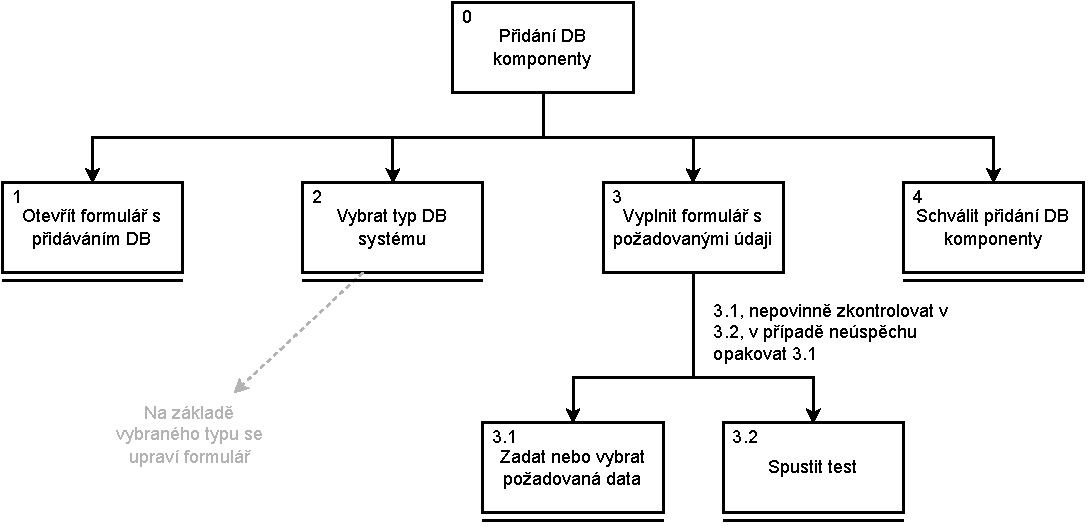
\includegraphics[height=70mm]{../img/HTA-1}
  \caption{Diagram pro přidání databázové komponenty.}
  \label{obr03:hta1}
\end{figure}

Kořen oznamuje jaký úkol bude uživatel provádět. V~první hladině máme kroky 1 až 4, které nám v~základních rysech ukazují, jak bude uživatel postupovat při plnění úkolu. Krok 3 dál rozdělíme na 3.1 Zadání dat a~3.2 Otestování. Na hraně pak definujeme postup uživatele při plnění kroků 3.1 a~3.2. Když není hrana popsaná, předpokládáme průběh kroků podle čísel v~hladině vzestupně. Konkrétní pořadí ale není podmíněné. Číslování 3 a~3.x vyjadřuje vztah mezi rodičem a~podúkoly.  Podtržené stavy v~HTA se dál nedělí. 

Takto vytvořený diagram nám neříká nic o~interakci uživatele s~konkrétním systémem. Díky tomu ale můžeme kroky rychle měnit a~upravovat. Lépe zhodnotíme, jestli uživatel nedělá příliš mnoho kroků pro dokončení úkolu, nebo naopak. Často se může stát, že jeden krok je ještě potřeba rozdělit.


\chapter{Storyboardy}

\todo[inline, color=blue!30]{Psaní v~procesu, zatím jen nápady.}

Na vytvoření uživatelských skupin a~HTA diagramů navážeme tvořením Storyboardů. Vezmeme vždy reprezentanta každé skupiny uživatelů a~představíme si jeho chování pro jednu vybranou situaci z~diagramu HTA.


Storyboard je náčrt sekvence kroků, které uživatel v~aplikaci provádí. Každý důležitý bod je zaznamenán do buňky. Ty pak skládáme lineárně za sebe, až nám vznikne příběh připomínající komiks. Takové rozdělení umožňuje soustředit se na každý krok zvlášť. Zároveň se jedná o~další techniku, kde můžeme udělat rychlý náčrt a~podle potřeby upravovat. Jeden storyboard nezabere víc než jednu stránku.

Takové grafické uchopení nám může dát první náznaky toho, jak by mohla aplikace vypadat. Nesnažíme se jít do detailů. Jde nám hlavně o~vizuální zobrazení kroků, které jsme popisovali v~HTA diagramech.

Storyboardy jsou nápomocné pro návrháře, aby si vizualizovali, jak budou uživatelé používat navrhovanou aplikaci. 

Technika storyboardů nebyla původně určena pro návrh uživatelského rozhraní. -> Ozdrojovat

Detail comes later zmínit


\chapter*{Závěr}
\addcontentsline{toc}{chapter}{Závěr}

\todo[inline, color=blue!30]{TODO: shrnout co se podařilo a co ne}

\todo[inline, color=blue!30]{TODO: Nezapomenout na konci nahradit mezery za no-break space všude v~dokumentu... pomocí \textasciitilde}

%%% Seznam použité literatury
%%% Seznam použité literatury (bibliografie)
%%%
%%% Pro vytváření bibliografie používáme bibTeX. Ten zpracovává
%%% citace v textu (např. makro \cite{...}) a vyhledává k nim literaturu
%%% v souboru literatura.bib.
%%%
%%% Příkaz \bibliographystyle určuje, jakým stylem budou citovány odkazy
%%% v textu. V závorce je název zvoleného souboru .bst. Styly plainnat
%%% a unsrt jsou standardní součástí latexových distribucí. Styl czplainnat
%%% je dodáván s touto šablonou a bibTeX ho hledá v aktuálním adresáři.

% \bibliographystyle{czplainnat}    %% Autor (rok) s českými spojkami
% \bibliographystyle{plainnat}    %% Autor (rok) s anglickými spojkami
\bibliographystyle{unsrt}       %% [číslo]

\renewcommand{\bibname}{Seznam použité literatury}

%%% Vytvoření seznamu literatury. Pozor, pokud jste necitovali ani jednu
%%% položku, seznam se automaticky vynechá.

\bibliography{literatura}

%%% Kdybyste chtěli bibliografii vytvářet ručně (bez bibTeXu), lze to udělat
%%% následovně. V takovém případě se řiďte normou ISO 690 a zvyklostmi v oboru.

% \begin{thebibliography}{99}
%
% \bibitem{lamport94}
%   {\sc Lamport,} Leslie.
%   \emph{\LaTeX: A Document Preparation System}.
%   2. vydání.
%   Massachusetts: Addison Wesley, 1994.
%   ISBN 0-201-52983-1.
%
% \end{thebibliography}


%%% Obrázky v bakalářské práci
%%% (pokud jich je malé množství, obvykle není třeba seznam uvádět)
\listoffigures

%%% Tabulky v bakalářské práci (opět nemusí být nutné uvádět)
%%% U matematických prací může být lepší přemístit seznam tabulek na začátek práce.
\listoftables

%%% Použité zkratky v bakalářské práci (opět nemusí být nutné uvádět)
%%% U matematických prací může být lepší přemístit seznam zkratek na začátek práce.
\chapwithtoc{Seznam použitých zkratek}

%%% Přílohy k bakalářské práci, existují-li. Každá příloha musí být alespoň jednou
%%% odkazována z vlastního textu práce. Přílohy se číslují.
%%%
%%% Do tištěné verze se spíše hodí přílohy, které lze číst a prohlížet (dodatečné
%%% tabulky a grafy, různé textové doplňky, ukázky výstupů z počítačových programů,
%%% apod.). Do elektronické verze se hodí přílohy, které budou spíše používány
%%% v elektronické podobě než čteny (zdrojové kódy programů, datové soubory,
%%% interaktivní grafy apod.). Elektronické přílohy se nahrávají do SISu a lze
%%% je také do práce vložit na CD/DVD. Povolené formáty souborů specifikuje
%%% opatření rektora č. 72/2017.
\appendix
\chapter{Přílohy}

\section{První příloha}

\openright
\end{document}
